\documentclass[11pt]{article}
\usepackage[margin=1in]{geometry}
\usepackage{graphicx}
\usepackage{amsmath,amssymb}
\usepackage{booktabs}
\usepackage{longtable}
\usepackage[colorlinks=true,linkcolor=blue,citecolor=blue,urlcolor=blue]{hyperref}
\graphicspath{{figs/}}

\newcommand{\vcut}{v_{\mathrm{cut}}}
\newcommand{\vmin}{v_{\mathrm{min}}}
\newcommand{\sobs}{\sigma_{\mathrm{obs}}}
\newcommand{\sborn}{\sigma_{\mathrm{Born}}}
\newcommand{\code}[1]{\texttt{#1}}

\title{\textbf{exclurad\_py: exact radiative corrections and target
straggling for exclusive meson electroproduction}\\[2mm]
\large Design, validation and the first $\pi^0$ production}
\author{V.~Kubarovsky\\ \small Jefferson Lab}
\date{\today}

\begin{document}
\maketitle

\begin{abstract}
\code{exclurad\_py} is an event generator for exclusive meson
electroproduction $ep\to e'\,h\,X$ covering $\pi^0$, $\eta$, $\rho$, $\phi$
and $J/\psi$ in one code, with exact first-order QED radiative corrections
built on EXCLURAD and with pre-vertex external radiation in the target. This
note is the evidence. The central result is that the generated event density
reproduces the exact calculation bin by bin without reweighting: over the
azimuth, where the correction swings from $1.15$ to $0.92$, events and
quadrature agree with $\chi^2/N=0.79$ over eighteen bins. The target radiator
is validated against an independent implementation, exclugen, to
$0.6\,\sigma$. Four independent samples on three machines, two processor
families and two python generations are statistically indistinguishable. The
note states, with equal care, what is \emph{not} yet established: the vector
channels have no external anchor for their radiative correction, and $\rho$
and $\phi$ still lack the Breit--Wigner mass, which for $\rho$ is not a
cosmetic omission.
\end{abstract}

\tableofcontents

\section{Scope and status}

The five channels are at different stages, and the difference matters more
than any single number in this note.

\begin{center}
\small
\begin{tabular}{lccc p{5.4cm}}
\toprule
channel & internal RC & external anchor & B--W mass & status \\
\midrule
$\pi^0$  & validated & published EXCLURAD table & n/a & production running \\
$\eta$   & validated & published table via $\vcut$ & n/a & next \\
$\rho$   & vs.\ own quadrature & none & \textbf{missing} & blocked on B--W \\
$\phi$   & vs.\ own quadrature & none & \textbf{missing} & blocked on B--W \\
$J/\psi$ & vs.\ own quadrature & none & not needed & box needs care \\
\bottomrule
\end{tabular}
\end{center}

``Validated against our own quadrature'' is a weaker statement than it sounds:
generator and reference share the same \code{rc\_factor}, so an error inside
that function is invisible to the comparison. It catches sampling errors,
which are the common ones, and cannot catch a wrong core. Only $\pi^0$ and
$\eta$ have something outside the code to lean on. This is why they come
first.

\section{The radiative correction}

EXCLURAD computes, in the Bardin--Shumeiko formalism, the observed cross
section for $ep\to e'h+X_{\rm miss}$ where the undetected system is
reconstructed by missing mass. The variable is the inelasticity
\begin{equation}
v \;=\; M_X^2(ep\to e'h) - m_U^2 ,
\end{equation}
zero for a non-radiative event. With an exclusivity cut $v<\vcut$,
\begin{equation}
\sobs(\vcut) \;=\; \sborn\,\bigl(1+\delta(\vcut)\bigr),
\end{equation}
and $\delta$ depends on all four hadronic variables and on the cut. Inside the
code the same quantity is stored as the multiplicative factor
$\eta=\sobs/\sborn$; the note quotes $\delta$ in that convention, so
$\delta\approx0.9$ means a $10\,\%$ suppression, not a $90\,\%$ one.

The soft and hard parts are separated at an arbitrary $\vmin$. Nothing
physical may depend on it, and §\ref{sec:vmin} shows that nothing does.

\section{How the correction is extracted from events}

Two runs of the same card differing only in \code{iborn} give
\begin{equation}
\delta(\mathrm{bin})=
\frac{N_{\rm rad}(\mathrm{bin})/N_{\rm rad}}
     {N_{\rm born}(\mathrm{bin})/N_{\rm born}}\times\frac{\sobs}{\sborn}.
\end{equation}
This is the whole method. Both samples come from the same generator, so the
ratio isolates the radiative machinery. Born events cost about a tenth of a
radiative one, so the Born sample is made five times larger and contributes
about a fifth of the variance.

\section{Proof: the correction over the azimuth}
\label{sec:proof}

The azimuth is the sharpest test available. The correction varies more over
$\phi$ than over any other variable, and $\phi$ is where a convention error
--- Trento or not, which hadron defines the plane, the sign of
$\sigma_{LT}$ --- shows up. Integrated quantities hide exactly these
mistakes.

\begin{figure}[htbp]
\centering
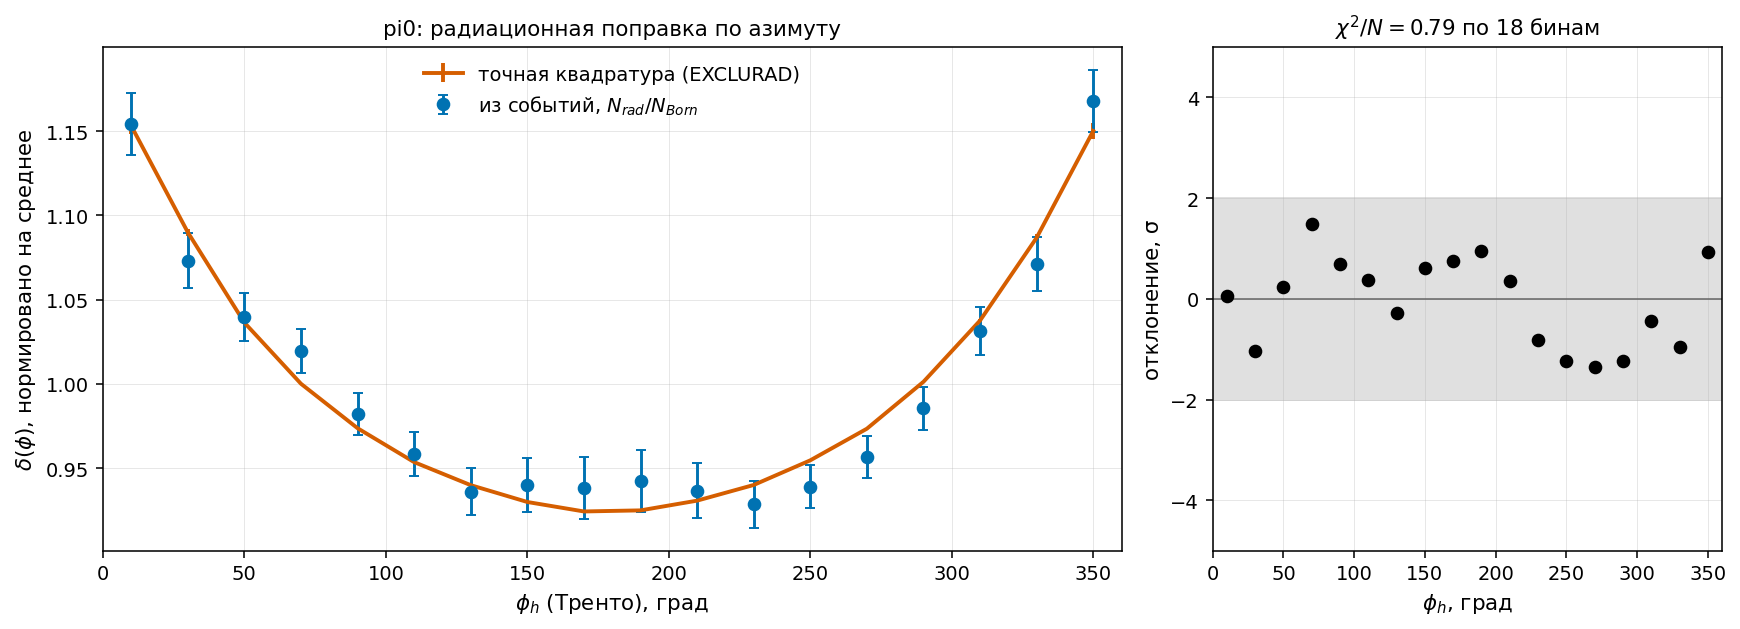
\includegraphics[width=\textwidth]{rc_proof_phi_pi0.png}
\caption{$\pi^0$, $E=10.6$~GeV, $Q^2\,1.5$--$2.5$, $W^2\,5.25$--$6.75$,
$|t|\,0.17$--$2.0$, $\vcut=0.20$~GeV$^2$, no target radiator.
Left: the radiative correction over the azimuth obtained two independent
ways --- from the events as the ratio of two histograms (points), and from
direct integration of the Bardin--Shumeiko formulas at the same kinematic
points (line). Right: the difference in standard deviations.
$100$k radiative and $500$k Born events; the quadrature uses $20$k points and
carries its own error, which is included in the pulls.}
\label{fig:proof}
\end{figure}

Figure~\ref{fig:proof} is the central result. The two determinations share no
machinery: one counts events, the other integrates formulas. They agree with
$\chi^2/N=0.79$ over eighteen bins, the largest deviation being $1.5\,\sigma$,
across a correction that swings by a quarter.

The practical consequence is that an analysis binning our events in $\phi$
recovers the exact correction by construction --- no reweighting, no
correction table.

\begin{center}
\small
\begin{tabular}{rccr}
\toprule
$\phi$ (deg) & from events & from quadrature & $\sigma$ \\
\midrule
 10 & $1.1542\pm0.0185$ & $1.1532\pm0.0046$ &  0.1 \\
 90 & $0.9822\pm0.0125$ & $0.9737\pm0.0003$ &  0.7 \\
170 & $0.9379\pm0.0184$ & $0.9242\pm0.0005$ &  0.7 \\
250 & $0.9390\pm0.0127$ & $0.9546\pm0.0003$ & $-1.2$ \\
350 & $1.1678\pm0.0185$ & $1.1501\pm0.0048$ &  0.9 \\
\bottomrule
\end{tabular}
\end{center}

\section{The same in the other variables}

\begin{figure}[htbp]
\centering
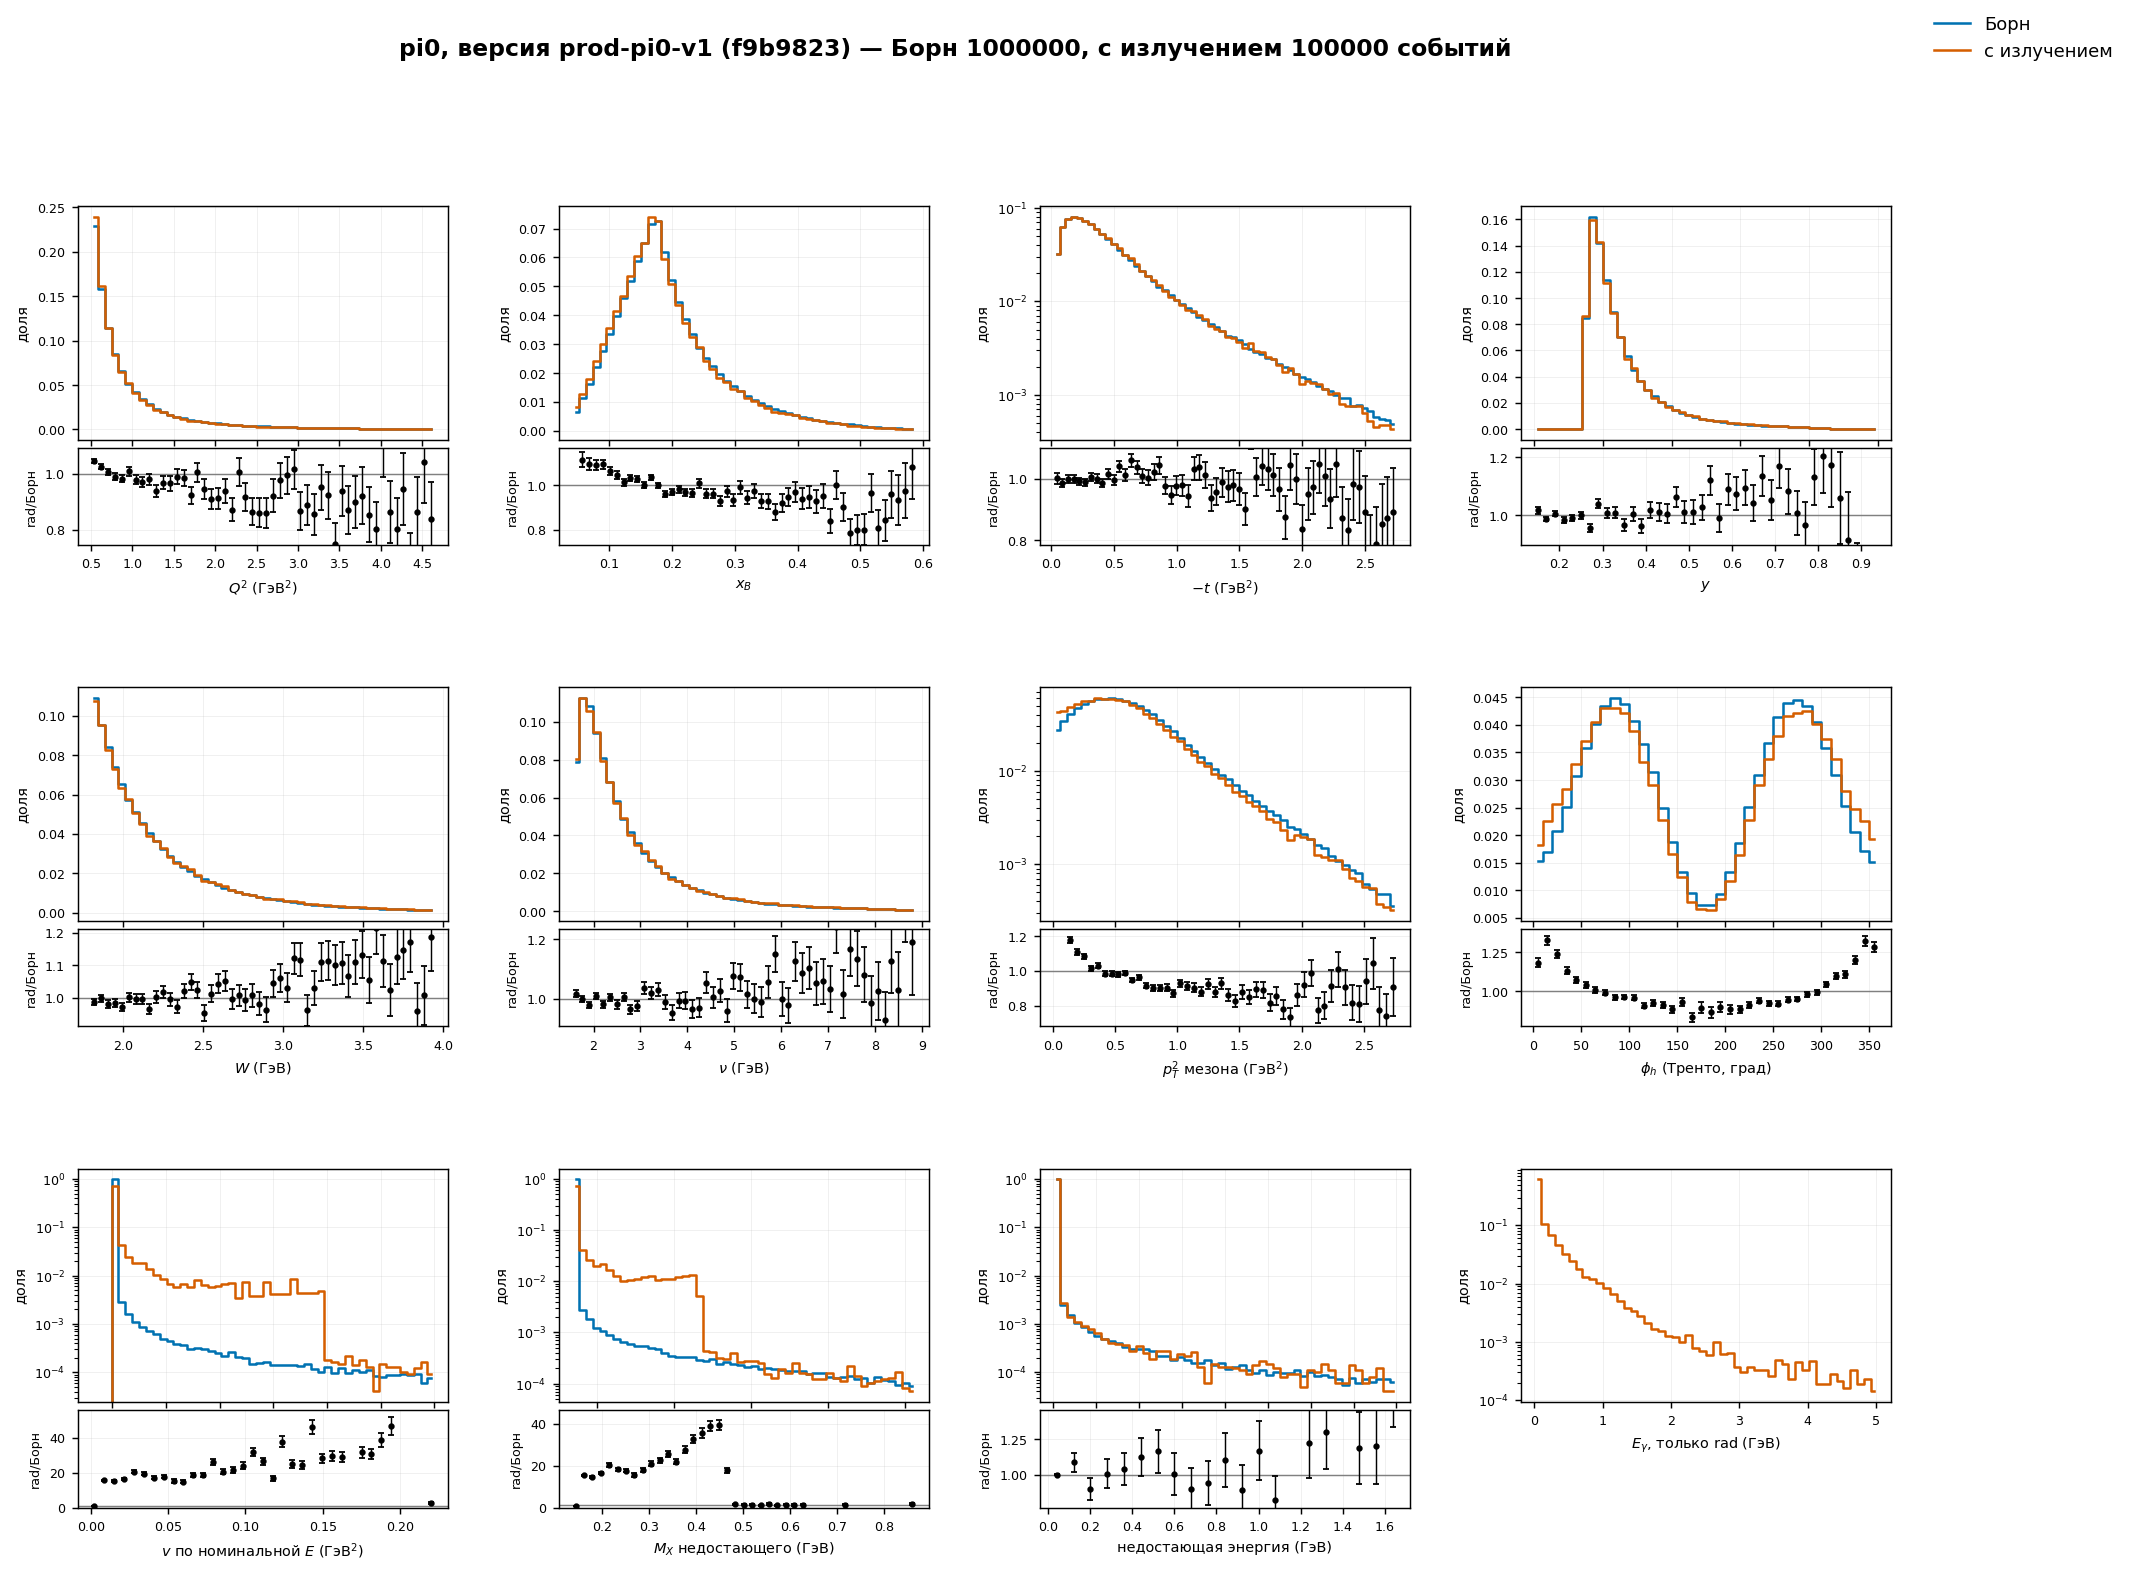
\includegraphics[width=\textwidth]{report_pi0.png}
\caption{$\pi^0$ production sample, radiator on. Upper half of each cell:
Born and radiative distributions normalised to unit area; lower half: their
ratio. The ratio is the correction as a function of that variable. Note the
inelasticity and missing-mass panels: the Born tail stops at the cut while
the radiative one extends, which is the radiative tail itself.}
\label{fig:report}
\end{figure}

Over the full production box the agreement with quadrature holds on every
axis. Measured on the $100$k union, maximum deviation in standard deviations
over twelve bins per axis:

\begin{center}
\small
\begin{tabular}{lcccc}
\toprule
channel & $Q^2$ & $W$ & $|t|$ & $\phi$ \\
\midrule
$\pi^0$   & 1.8 & 1.9 & 1.7 & 2.0 \\
$\eta$    & 2.0 & 1.6 & 1.9 & 2.6 \\
$\rho$    & 2.7 & 1.5 & 2.8 & 1.6 \\
$\phi$    & 2.1 & 2.7 & 1.4 & 1.9 \\
$J/\psi$  & 2.9 & 3.0 & 1.7 & 1.9 \\
\bottomrule
\end{tabular}
\end{center}

At twelve bins the worst of twelve is expected around $2.5\,\sigma$ purely by
chance, so these numbers are what agreement looks like.

\section{Independence of the soft/hard separator}
\label{sec:vmin}

$\vmin$ splits the tail integral into an analytic soft part and a numerical
hard part. Moving it by two orders of magnitude moves half the contribution
from one to the other, and the total must not notice.

\begin{center}
\small
\begin{tabular}{lccc}
\toprule
$\vmin$ (GeV$^2$) & $\sobs$ (nb) & hard fraction \\
\midrule
$10^{-5}$ & $0.026400\pm0.000088$ & 51.3\,\% \\
$10^{-4}$ & $0.026121\pm0.000068$ & 42.1\,\% \\
$10^{-3}$ & $0.026236\pm0.000087$ & 32.5\,\% \\
\bottomrule
\end{tabular}
\end{center}

The hard fraction changes by a factor of $1.6$; the cross section is constant
to $1.1\,\%$, with the largest pairwise difference at $2.5\,\sigma$. There is
no monotonic trend --- the middle value lies below both ends --- so this looks
like statistics rather than a residual dependence. It is honest to say that
$2.5\,\sigma$ is ``not caught'' rather than ``clean''; separating a
half-percent systematic from a fluctuation needs four times the statistics.

\section{External radiation in the target}
\label{sec:ext}

An electron crosses part of the target before interacting and radiates on the
way in. Geant4 cannot supply this: it starts at the vertex and takes the beam
energy as given, so the incoming leg is the generator's responsibility and
nothing in the CLAS12 chain was providing it. The outgoing leg is deliberately
\emph{not} modelled here --- Geant4 does it, and doing it twice is worse than
not doing it at all.

The sampling follows exclugen and aao\_rad: the vertex is uniform over the
cell, $bt=(4/3)(v_z-v_{z,\min})/X_0$ with $X_0(\mathrm{LH_2})=890.4$~cm, and
the surviving energy fraction is $u^{1/bt}$. Against the analytic straggling
law over $400$k draws: $P(\mathrm{loss}>1\,\%)$ is $1.674\,\%$ against
$1.704\,\%$, and $P(\mathrm{loss}>10\,\%)$ is $0.818\,\%$ against $0.857\,\%$.

\paragraph{Validation against an independent implementation.}
The observable effect is that events are pushed out of the exclusivity
window, because an analysis reconstructs the missing mass with the
\emph{nominal} beam energy. Running exclugen twice, with and without its own
radiator, over six independent pairs of $600$k events gives a shift of
$0.873\pm0.112\,\%$ in the cut efficiency. Our generator, measured the same
way:

\begin{center}
\small
\begin{tabular}{lcc}
\toprule
source & fraction above the cut & events \\
\midrule
mac mini            & $0.865\pm0.047\,\%$ & 40k \\
JLab farm           & $0.771\pm0.031\,\%$ & 80k \\
combined            & $\mathbf{0.800\pm0.026\,\%}$ & \\
exclugen (reference)& $0.873\pm0.112\,\%$ & $6\times600$k \\
\bottomrule
\end{tabular}
\end{center}

Agreement at $0.6\,\sigma$, and with the radiator off, exactly zero events out
of forty thousand lie above the cut. This is the first piece of our physics
checked against somebody else's code rather than against our own quadrature.

One measurement lesson is worth recording. The scatter between exclugen pairs
($0.275\,\%$) exceeds the binomial error of a single pair ($0.177\,\%$),
because exclugen rebuilds its sampling ceiling from a prescan each run. The
first two pairs gave $-1.20$ and $-0.44\,\%$ and disagreed by three standard
deviations; both were correct and both were useless alone.

\paragraph{What this means for the user of the sample.}
With the radiator on, $\vcut$ is applied in \emph{true} variables. About
$0.8\,\%$ of the delivered events will fail an exclusivity cut made with the
nominal beam energy --- for Born events too, since the electron loses energy
before the vertex whatever happens there. The sample is nevertheless complete:
\begin{equation}
v_{\rm rec}-v_{\rm true}=2\,\Delta E\,(E_X-p_{X,z})\;\ge\;0 ,
\end{equation}
so external loss can only move events out of the window, never into it.

\section{Reproducibility}
\label{app:mach}

\begin{figure}[htbp]
\centering
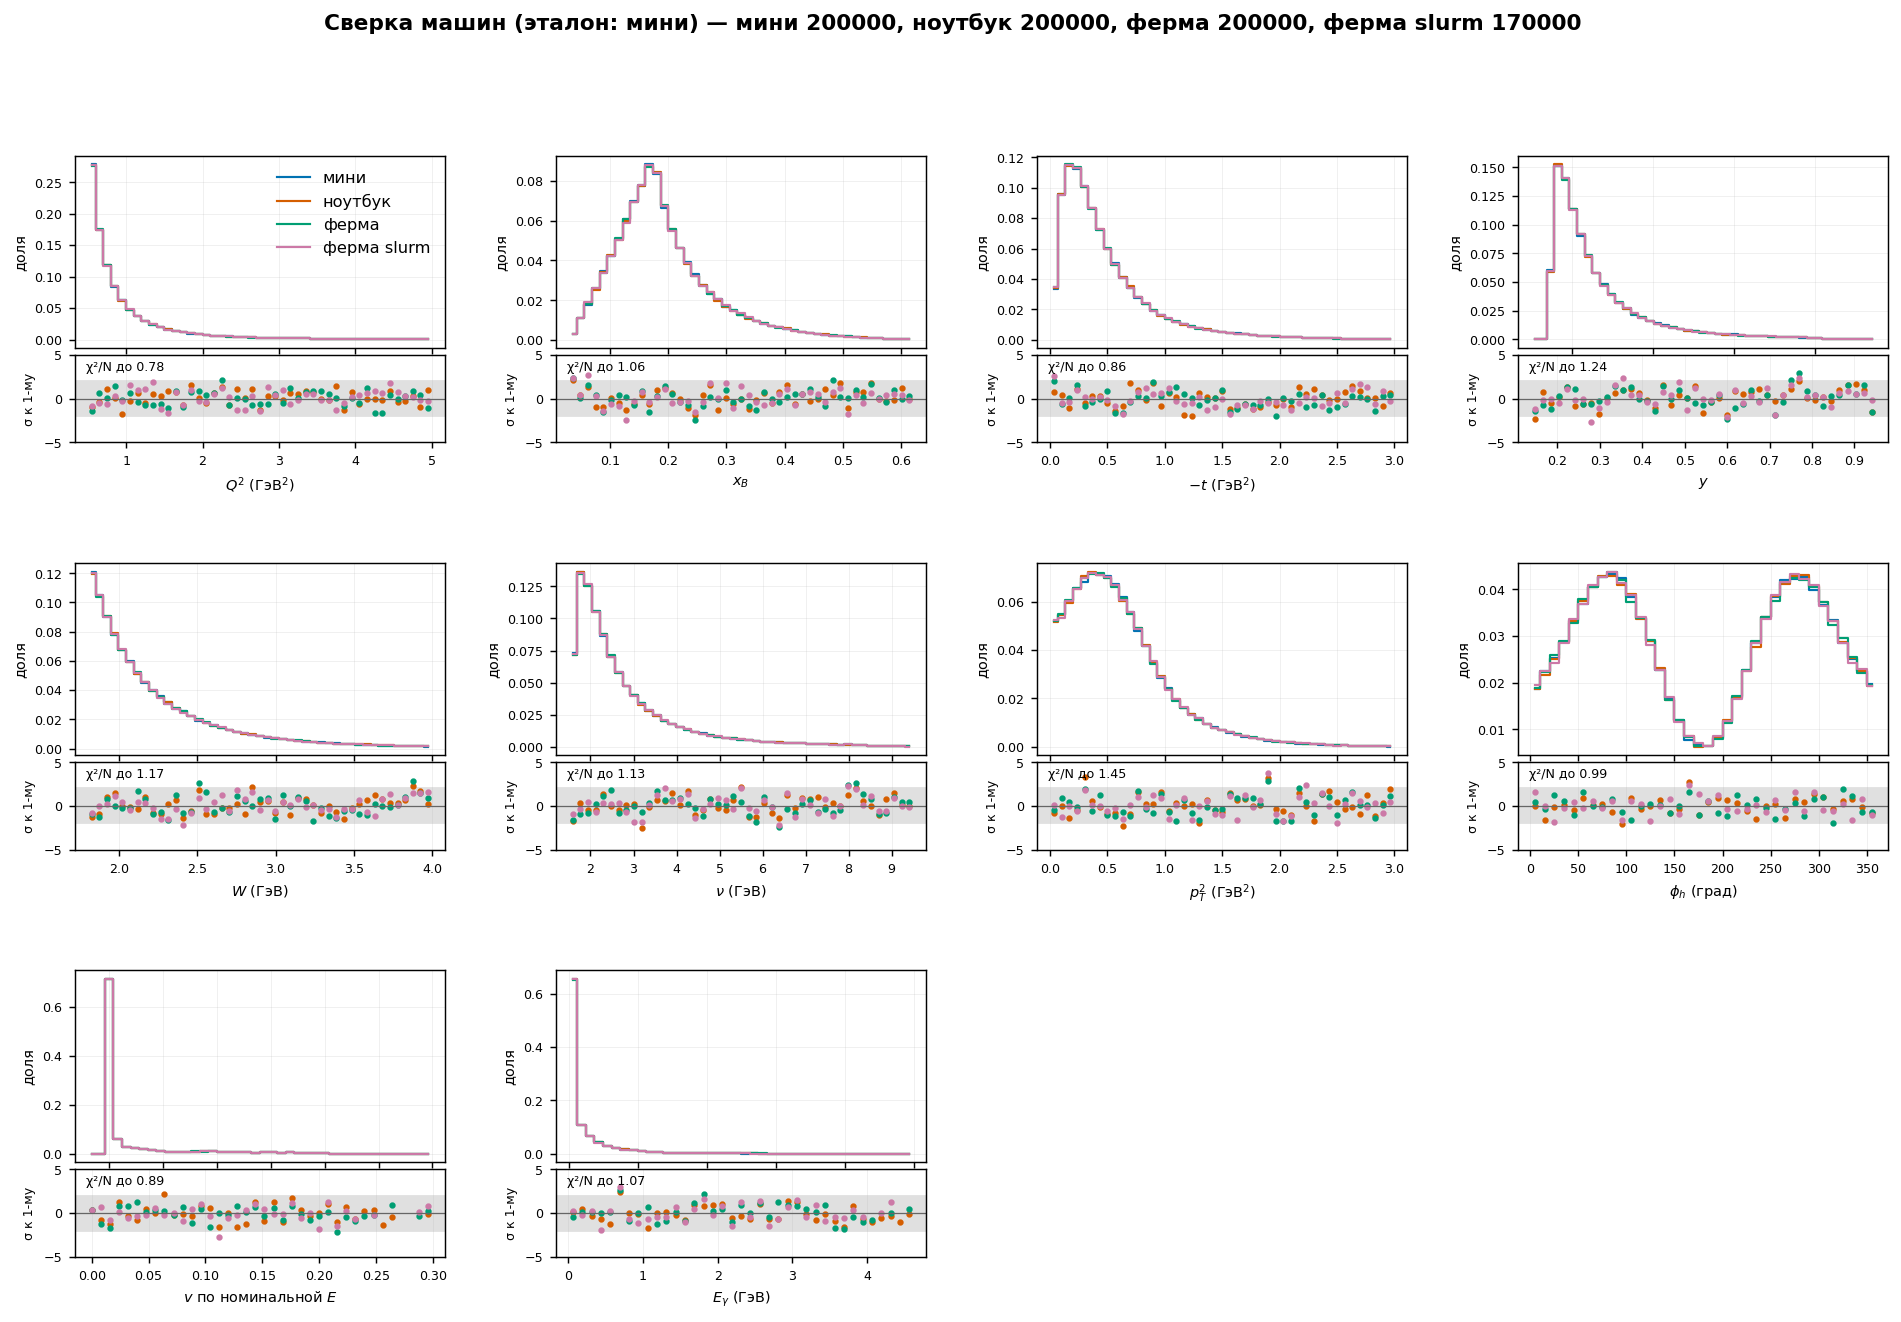
\includegraphics[width=\textwidth]{machines.png}
\caption{Four independent samples: mac mini (M4), MacBook Pro (M3 Max), the
JLab farm interactively and the same farm through slurm. Different seeds,
different processors, python 3.9 with numpy 1.23 against python 3.14 with
numpy 2.4. Lower panels: deviation from the first sample in standard
deviations, grey band $\pm2\sigma$.}
\label{fig:machines}
\end{figure}

The worst $\chi^2/N$ over ten variables is $1.45$ ($p_T^2$) and the median is
about $1.1$. Nothing in the chain --- processor, library version, interactive
versus batch --- leaves a trace in the sample. Two further checks: a run
repeated with the same seed reproduces its output byte for byte, and $100$k
events pooled from two machines contain exactly $100$k distinct events.

\section{Output integrity}

Conservation laws are checked per event rather than inferred from the shape of
a distribution: the header's particle count, four-momentum against beam plus
target over the status-1 particles, mass shells, the written mass against PDG,
decay closure, charge, and the beam-polarisation column. All five channels
pass; four-momentum closes to $1.25\times10^{-8}$~GeV and the decay to
$10^{-10}$, both far inside the $10^{-6}$ tolerance.

\section{What is not established}

\paragraph{The vector channels have no external anchor.} $\rho$, $\phi$ and
$J/\psi$ are checked against our own quadrature only. DIFFRAD, the
Akushevich code for vector mesons, is on disk and is the natural reference;
this comparison has not been made.

\paragraph{$\rho$ and $\phi$ have no Breit--Wigner mass.} The meson is
generated exactly on the pole. For $\phi$, $\Gamma/M=0.4\,\%$ and this is
below resolution; for $\rho$, $\Gamma=150$~MeV at $M=775$~MeV, and a fixed
mass is wrong in a way that matters. The mass enters the $t$ limits, the $W$
threshold and through them the region where the correction is evaluated, so
this is not only the shape of the peak. The sampler has been ported from
\code{diffrad\_vm.f90} and agrees with it ($\chi^2/N=0.80$ for $\rho$, $0.73$
for $\phi$ over $200$k draws each); what remains is to make the mass a
property of the event throughout the kinematics.

\paragraph{$\rho$ and $\phi$ run with no inelasticity cut.} $\vcut=0$ by
decision, meaning the tail runs to the kinematic limit where the diffractive
model is extrapolated far outside its fit. With $\vcut=0$ the $\rho$
correction carries an $8\,\%$ slope in $Q^2$ that the quadrature does not
have ($\chi^2/N=4.04$); at $\vcut=0.20$ the slope is gone ($2.04$).

\paragraph{$\pi^0$ table interpolation.} The interpolation rms is $0.029$
against a tolerance of $0.02$, and refining does not help: $1000\to6144$
nodes moves it from $0.029$ to $0.027$, while the other four channels sit at
$0.002$--$0.006$. Correctness is unaffected --- the second stage is exact ---
but efficiency is.

\paragraph{The exponentiation systematic} is measured but not resolved:
$\delta$ with and without the YFS exponentiation differs by $-0.66\,\%$
($\pi^0$), $-0.48\,\%$ ($\eta$), $-1.47\,\%$ ($\rho$), $-1.44\,\%$ ($\phi$)
and $-0.09\,\%$ ($J/\psi$). It should be quoted as a theory systematic.

\section{Summary}

For $\pi^0$ the generator is ready: the event density reproduces the exact
calculation over the azimuth to $\chi^2/N=0.79$, the target radiator agrees
with an independent implementation to $0.6\,\sigma$, four samples on three
machines are indistinguishable, and the output satisfies the conservation
laws event by event. $\eta$ shares the machinery and needs its own production
and its own published-table comparison. The vector channels need the
Breit--Wigner mass first --- mandatory for $\rho$ and $\phi$ --- and then an
external anchor, for which DIFFRAD is available and unused.

\end{document}
